
\documentclass{article}
\usepackage{amsmath}
\usepackage[utf8]{inputenc}
\usepackage{subfig}
\usepackage{graphicx}

\usepackage{amsbsy}
\usepackage{hyperref}
%\title{Deep Reinforcement Learning for Perspective Taking Task}
\title{Perspective-Taking Using Deep Reinforcement Learning}
\author{Aqeel Labash}
\date{September 2017} 
\usepackage{natbib}
\usepackage{graphicx}
\usepackage{makecell}
\usepackage{float}
\usepackage[%
    left=1.0in,%
    right=1.0in,%
    top=1.0in,%
    bottom=1.0in,%
    paperheight=11in,%
    paperwidth=8.5in%
]{geometry}%
\begin{document}
\maketitle
\section*{Abstract}
Perspective taking is the ability to take the point of view of another agent. This capability is not unique to humans but it is also displayed by other animals like chimpanzees. It is an essential ability to achieve efficient social interactions, including cooperation and competition. In this work, we present our progress toward building artificial agents with such abilities. To this end we created perspective-taking tasks, in which the environment is partially observable by agents who compete for a common resource. We show that agents controlled by artificial networks learn via reinforcement learning to pass multiple tests that would benefit from perspective taking capabilities. We believe that the building of artificial agents with perspective taking faculties might help to reverse engineering how perspective taking task might be accomplished in our brains.


\section{Introduction}
Many decisions we take depend on others, what they think, what they believe, and what we know about what they know. This ability to understand and infer the mental states of others is called \textit{theory of mind} \cite{premack1978does} or mindreading \cite{apperly2011mindreaders}. Not only humans have the ability to take into consideration what others think and believe. In controlled experiments, it has been shown that chimpanzees can know what other conspecifics see and know \cite{hare2000chimpanzees}. Here we ask whether artificial intelligence (AI) agents controlled by neural networks could also learn to infer what other agents perceive and know. In particular, we test here the ability of an agent trained via reinforcement learning to acquire one essential part of \textit{theory of mind}: perspective taking. 

Perspective taking is looking at things from a perspective that differs from our own \cite{ryskin2015perspective}. It could be defined as "the cognitive capacity to consider the world from another individual's viewpoint" \cite{davis1983measuring}. According to Galinsky and colleagues, it is one of the social competencies that motivates social understanding in many contexts \cite{galinsky2008pays}.

\par When two persons are in a room that is familiar to both of them, they do not need to switch places to imagine what another can see and cannot see. However, this perspective taking ability is not unique to humans but it has been observed in other animals like chimpanzees \cite{hare2000chimpanzees}. Chimpanzee social status is organized hierarchically (dominant, subordinate) \cite{goldberg1997genetic}. When there is food available that both can reach, the dominant almost always gets it. In the experiments \cite{hare2000chimpanzees}  two chimpanzees were set into two separate cages facing the other with food positioned between them as shown in Figure \ref{tom.experiment} (left). The three conditions differed mainly in what the dominant and the subordinate can see. For example in the "subordinate door" condition one piece of food cannot be seen by the dominant chimpanzee. Can the subordinate take advantage of this fact? The results are shown in Figure \ref{tom.experiment} (right) and demonstrated that the subordinate indeed obtained more food in this condition. Hence, the subordinate was able to take into account what the dominant chimpanzee could see. In other words, the subordinate could take the perspective of the dominant chimpanzee. For other experiments and details see for example \cite{hare2000chimpanzees, de2016we, tomasello2009cultural}.  

\begin{figure}[!ht]
\begin{center}
\includegraphics[scale=0.3]{figures/tom_experiment_1.png}
\includegraphics[scale=0.3]{figures/tom_experiment_1_results.png}
\caption{Left: three different positions for the food with different ability to observe it (food indicated by black ellipses, cage walls indicated by lines). Right top: Average percentage of eaten food by subordinate between different food positions. Right bottom: the average percentage based on food visibility condition. \cite{hare2000chimpanzees}}
\label{tom.experiment}
\end{center}
\end{figure}

We designed an environment \texttt{APES} that allowed us to simulate experiments in \cite{hare2000chimpanzees} where a subordinate chimpanzee chose whether to go for food or not depending on the observability of the food by the dominant chimpanzee. The aim of the present work is to study whether an AI agent controlled by a neural network can learn to solve similar perspective taking task using reinforcement learning (RL).

RL is a branch of AI that allows an agent to learn by trial and error while interacting with the environment. In particular, the agent must learn to select the best action in each specific state to maximize its cumulative reward \cite{sutton1998reinforcement}. The agent could be an autonomous robot \cite{lin1993reinforcement,yang2004multiagent,riedmiller2009reinforcement} or a character in video game \cite{mnih2013playing,tampuu2017multiagent} or even computer simulations based of biological systems \cite{amigoni2007multiagent}. 

\par 
The idea behind learning by interacting with an environment is inspired from how human and animal infants learn from the rich cause-effect or action-consequence structure of the world \cite{sutton1998reinforcement,thorndike1911animal,schultz1997neural}. Therefore, RL is a biologically plausible method of learning certain associations and behavior. 

We do not think that RL captures all aspects of perspective taking or is the exact model how perspective taking is learned in biological organisms (Aru \& Vicente, submitted). However, we hope that understanding the capabilities and limitations of RL in acquiring perspective taking skills will lead to a better algorithmic understanding of perspective taking in biological organisms.
\subsection{Related work}

\section{Methods}
To train a model capable of solving tasks that require perspective taking, three ingredients were needed. First, an environment to simulate the task. Second, a neural network model. Third, a training strategy for acquiring perspective taking since its not a straightforward task to be learned end to end.
\subsection{Environment}
%\textbf{General speaking about the envrionment functionality like you can use 10 agents etc .. }
To create our experiments we used Artificial Primate Environment Simulator (\textit{APES}) which contains features like multi-agents possibility, partial observability and binary environment representation \cite{APES}. \textit{APES} allow to build vision barriers (obstacles) and calculate vision based on agents location, orientation and vision range. For more details the reader can access the \href{https://github.com/aqeel13932/APES}{GitHub repository}

We created an $11\times11$ grid world environment. The elements in the world have certain places to spawn in, in every episode with Driclicht distribution. Figure (\ref{fig:probabilities}) show the elements possible locations at the beginning of every episode. In all experiments that have a dominant agent \(A_{dom}\) it always move in random steps toward unexplored area. Once \(A_{dom}\) spot the food (reward) it move toward it immediately (deterministic algorithm).
\begin{figure}[H]
    \centering
    \includegraphics[scale=0.5,trim={0cm 1cm 0cm 0cm},clip]{figures/probabilities.png}
    \caption{Show the possible start position for each element in the environment. Agent 1: is the subordinate, Agent 2 is the dominant.(Best seen with colores)}
    \label{fig:probabilities}
\end{figure}

\subsection{Model}
We kept the model simple and straight forward. We used a feedforward neural network \cite{Goodfellow-et-al-2016}. Our model estimate state value, and advantages which is similar to dueling network \cite{DBLP:journals/corr/WangFL15} but instead of splitting the last layer we used all of it for value and advantages. Figure \ref{fig.model} shows our model. In our task no convolutional neural networks were used. Each experiment generated two models: 1) training model, which is updated every time step, 2) target model which $\tau$-averaged copy of training model weights every step (\(\theta^{-} = \theta \times \tau + \theta^{-} \times (1-\tau)\)).
  \begin{equation} \label{eq:model.mod}
    Q(s,a;\theta,\alpha,\beta) = V(s;\theta,\beta) +\left( A(s,a;\theta,\alpha) - \underset{a' \in |A|}{\max}A(s,a';\theta,\alpha) \right)
  \end{equation}
\begin{figure}[!ht]
\begin{center}
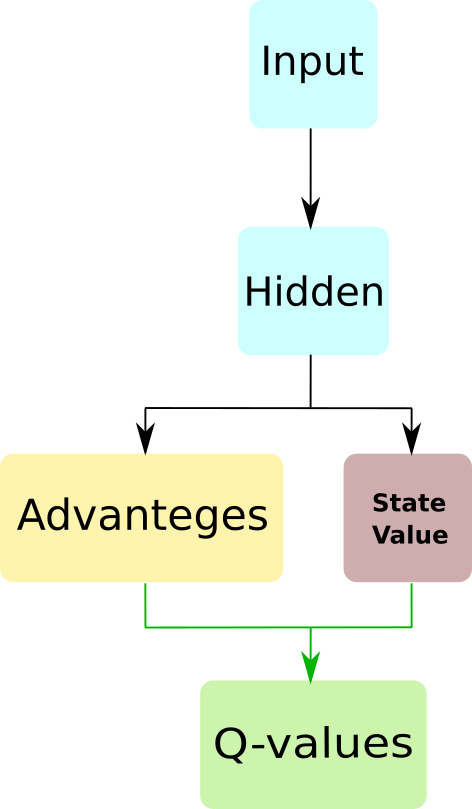
\includegraphics[scale=0.5]{figures/model1.png}
\caption{Feedforward network where the connections between the last layer and the Q-values is regulated by formula \ref{eq:model.mod}}
\label{fig.model}
\end{center}
\end{figure}

 \par We fed \label{network.input} agent visual field as input to the agent's network in the form of binary feature vectors. Separate binary map was used for agent position, dominant agent position, food position, observed area and obstacles position. In addition one-hot vector of size 4 for each agent was added to represent agent's direction.

\par We used replay memory or experience replay which is a common practice when deep learning is used for RL tasks\cite{DBLP:journals/corr/WangFL15,mnih2015human,mnih2013playing}. Replay memory is a set of transitions (\(s_t,r_t,a_t,s_{t+1},terminal\)) which is used to train the network.

\subsection{Perspective-taking Task}
The task we used included two agents: dominant $A_{dom}$ and subordinate $A_{sub}$. $A_{dom}$ and $A_{sub}$ are placed in an arena that contain obstacles $O$ that block vision and food $F$ which is the reward. The $A_{sub}$  need to get the food while keeping certain distance from dominant, otherwise it will be punished. $A_{dom}$ is driven by deterministic algorithm to find the food. 
We trained our agent in a curriculum learning scheme.
Curriculum learning consist of training an agent on a sequence of tasks of increased complexity to improve the speed of learning in a more complex task \cite{narvekar2016curriculum}. We defined tw tasks explained in the following sections where trained the agent first to find the food (Task 1) after that to avoid the dominant (Task 2).
\subsubsection{Task 1: finding the food} \label{task1}
In this stage the only task \(A_{sub}\) had was to find the food and eat it. This task might look easy but when we consider the vision and the obstacles it gets more complicated. Without a memory the agent has to act depending on the immediate vision of field. This task optimize \(A_{sub}\) to look for the food and approach it. To make the task reasonable, the obstacle will spawn randomly in specific region as shown in Figure \ref{fig:probabilities}. In this task the input representing dominant agent is zeros. The agent receives a -0.1 per time step regardless of the chosen action and 1000 for consuming food.
\subsubsection{Task 2: avoiding dominant agent}\label{task2}
Here, we trained the subordinate agent with a punishing dominant agent. The dominant gave -100 reward points for the subordinate whenever the subordinate was 1 steps away from the dominant and in its field of vision. 
 
\subsection{Behavioral test cases}\label{agents.behavior}
We created 10 behavioral tests cases where none of them can be accomplished without perspective taking. In those test cases we tried to cover all the possible factors. Mainly we stabilized all elements (dominant, subordinate, food, obstacle) positions with exception of one of them at a time.
In addition to different types we tried 5 variation of each test case to make sure that results weren't just a statistically calculated. The test cases can be found 

\begin{itemize}

\item \textbf {Test case 1:} in this test the subordinate agent \(A_{sub}\) optimally supposed to go for the food since the food is unobserved by the dominant agent \(A_{dom}\). At the same time \(A_{sub}\) cannot see \(A_{dom}\). Environment in Figure (\ref{fig.tc.1}).

\item \textbf {Test case 2:} \(A_{sub}\) can see the food and \(A_{dom}\). The favored behavior from \(A_{sub}\) is to avoid the food since \(A_{dom}\) can see the food. Environment in Figure (\ref{fig.tc.2})

\item \textbf {Test case 3:} \(A_{sub}\) supposed to go for the food in case \(A_{dom}\) was not spotted in its field of vision before eating the food. Environment in Figure (\ref{fig.tc.3}).

\item \textbf {Test case 4:} \(A_{sub}\) and \(A_{dom}\) can see each other while only \(A_{sub}\) can see the food. Hence, \(A_{sub}\) supposed to go for the food. Environment in Figure \ref{fig.tc.4}.

\item \textbf {Test case 5:} similar to test case 2 where \(A_{sub}\) with exception that \(A_{dom}\) is more distanced from the food. Environment in Figure (\ref{fig.tc.5})

\item \textbf {Test case 6:} agents can see each other but only \(A_{sub}\) can see the food. Similar case to Figure \ref{fig.tc.4} but \(A_{dom}\) here is closer to food. The expected behavior is to go for the food. Environment in Figure \ref{fig.tc.6}.

\item \textbf {Test case 7:} agents can see the food but not each other. \(A_{sub}\) should go to food as long as \(A_{dom}\) is not spotted before taking the last action. Environment in Figure \ref{fig.tc.7}

\item \textbf {Test case 8:} \(A_{sub}\) can see both food and \(A_{dom}\) while the latter cannot see neither \(A_{sub}\) nor the food. \(A_{sub}\) supposed to go for the food as the dominant is looking away. Environment in Figure \ref{fig.tc.8}.

\item \textbf {Test case 9:} \(A_{sub}\) see all other elements while \(A_{dom}\) does not.\(A_{sub}\) supposed to go for the food. Environment in Figure \ref{fig.tc.9}

\item \textbf {Test  case 10:} \(A_{sub}\) and \(A_{dom}\) can see the food, but can not see each other. Figure \ref{fig.tc.10}
\end{itemize}




\subsection{Training}
We trained our models on curriculum learning. First we trained it on task 1 for 2 million steps and exploration 1 which decrease to reach 0.1 after 1,5 million steps. Afterward we trained the model on task 2 for 500k step with exploration 0.1 from the beginning. We explored many values for hyper-parameters showin Table \ref{tab:best.hyp}. Typically we ran grid search procedure for different combinations of pairs of parameters.
\par Choosing the best hyper-parameters was based on the training average reward over multiple random seeds. Table \ref{tab:best.hyp}  show the best hyper-parameters that fit our task. For neural network implementation we used \texttt{Keras} library \cite{chollet2015keras}.

\begin{table}[H]
    \centering
    \begin{tabular}{*{2}{|c|}}
    \hline
         \textbf{Replay memory size}& 100K\\
         \hline
         \textbf {\# layers }&1\\
         \hline
         \textbf {Hidden nodes}&100\\
         \hline
         \(\boldsymbol{\tau}\)&0.001\\
         \hline
         \textbf {Advantage}&\texttt{max} \\
         \hline
         \textbf {Activation}&\texttt{tanh}\\
         \hline
         \(\boldsymbol{\epsilon}\)&0.01\\
         \hline
         \textbf {Batch size}&32\\
         \hline
         \textbf {Training repeat} &1\\
    \hline
    \end{tabular}
    \caption{best hyper-parameters}
    \label{tab:best.hyp}
\end{table}

Those hyper-parameters performed the best over multiple random seeds. We used them for the rest of the experiments.

\section{Results}

\subsection{Behavioral test cases}
Our goal is to study whether deep RL agents could learn to infer what other agents can and cannot perceive. We tested our agents with 10 test cases designed to be accomplished only with perspective taking abilities. In those test cases we paused the dominant movement completely to see the emerged behavior from the subordinate. The following figures illustrate the test cases and the agent's behavior. The legend of each figure explains the situation and the behavior in more detail.

\begin{figure}[H]
    \centering
    \subfloat[]{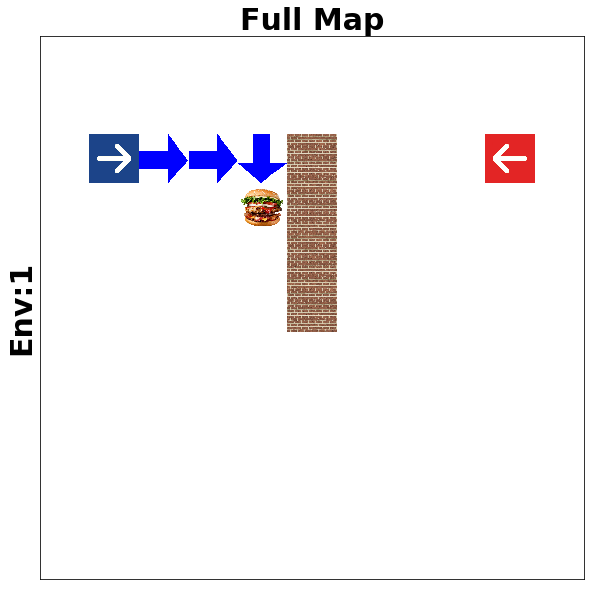
\includegraphics[scale=0.20]{figures/ENV:1_FM.png}}
    \subfloat[]{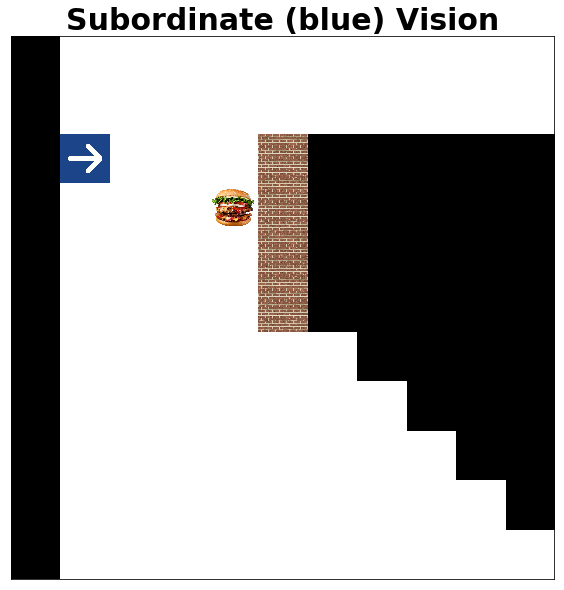
\includegraphics[scale=0.20]{figures/ENV:1_AI.png}}
    \subfloat[]{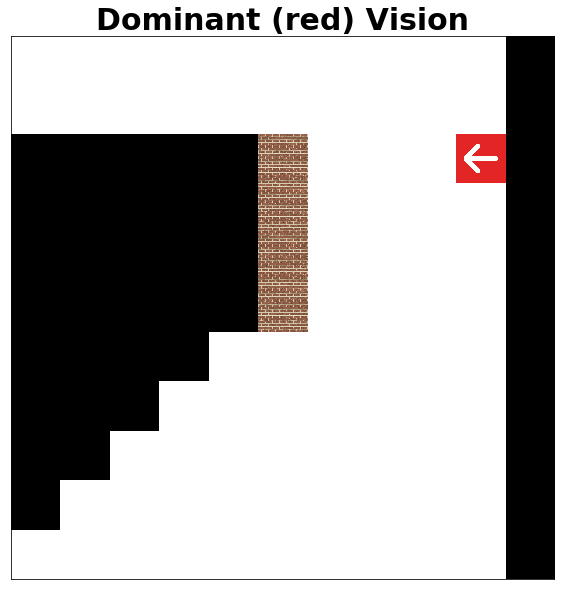
\includegraphics[scale=0.20]{figures/ENV:1_DM.png}}
    \caption{\textbf {Test  case 1:} \(A_{sub}\) did not see the dominant as the dominant was behind the obstacle. The subordinate \(A_{sub}\) went for the food in 6 steps. The followed path was optimal.  For this test case the agent achieved the expected behavior.}
    \label{fig.tc.1}
\end{figure}

\begin{figure}[H]
\begin{center}
\subfloat[]{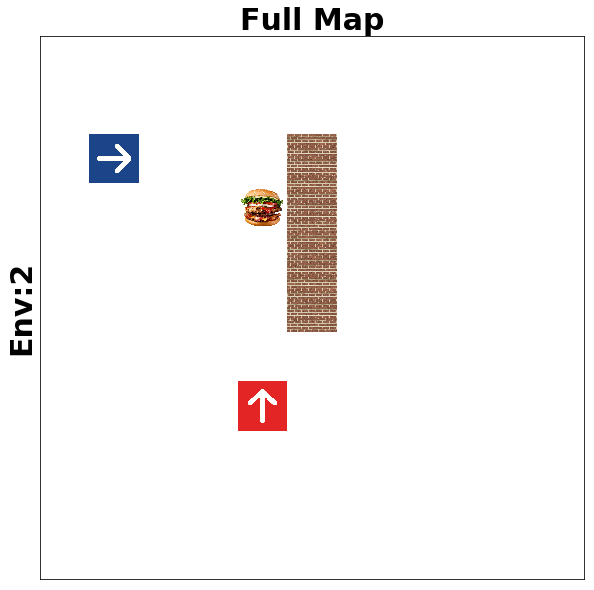
\includegraphics[scale=0.20]{figures/ENV:2_FM.png}}
\subfloat[]{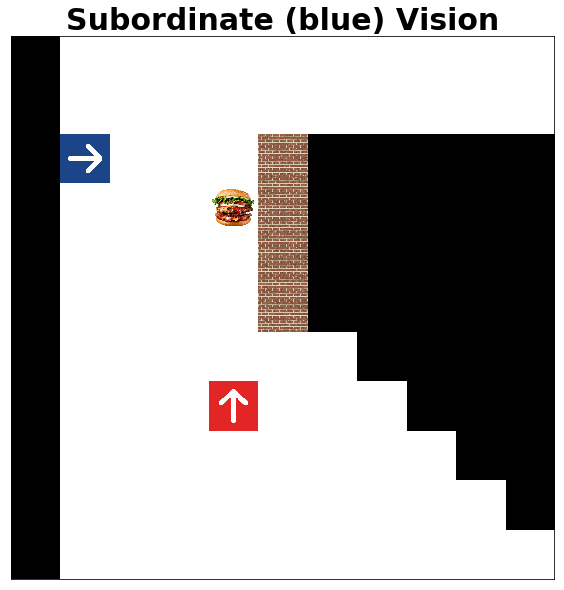
\includegraphics[scale=0.20]{figures/ENV:2_AI.png}}
\subfloat[]{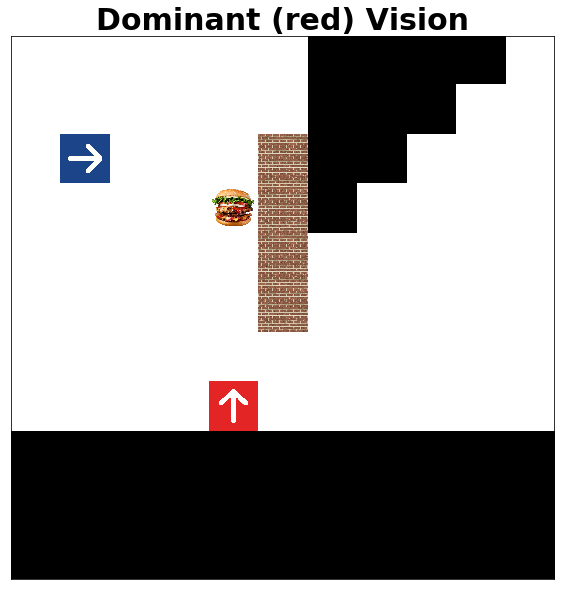
\includegraphics[scale=0.20]{figures/ENV:2_DM.png}}
    \caption{Test  case 2: \(A_{sub}\) avoided the food although the food is in the same position as in \texttt{Test case 1}. The only difference is the dominant position and direction: the dominant can see the food. The observed behavior is also what one would expect from an agent with the perspective taking ability.}
    \label{fig.tc.2}
\end{center}
\end{figure}
\begin{figure}[H]
\begin{center}
\subfloat[]{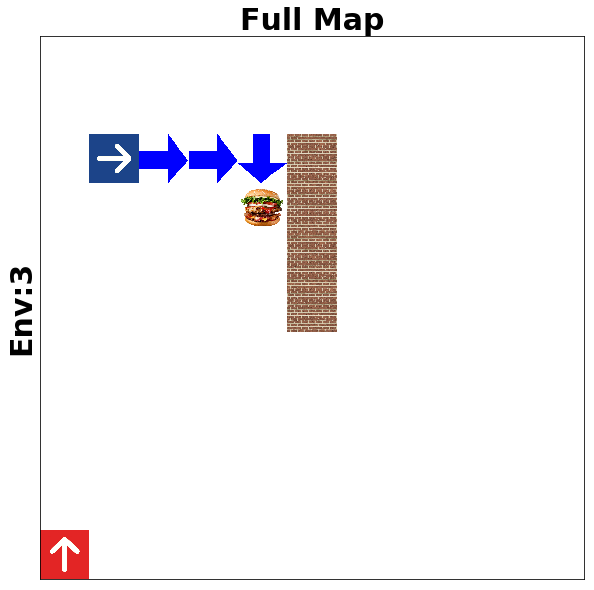
\includegraphics[scale=0.20]{figures/ENV:3_FM.png}}
\subfloat[]{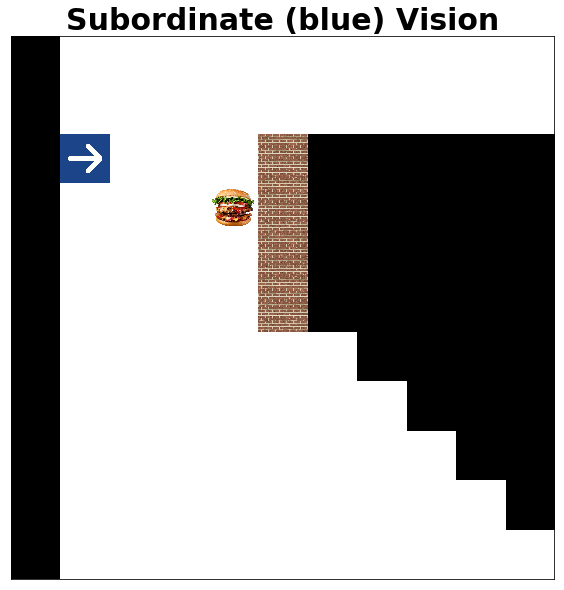
\includegraphics[scale=0.20]{figures/ENV:3_AI.png}}
\subfloat[]{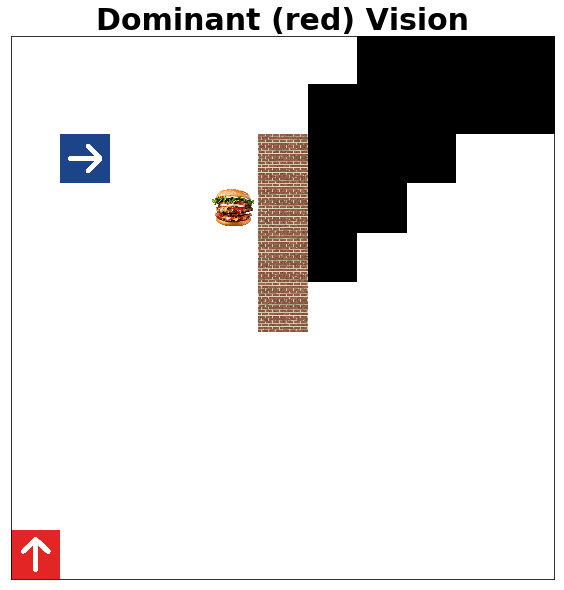
\includegraphics[scale=0.20]{figures/ENV:3_DM.png}}
\caption{Test  case 3: \(A_{sub}\) went for the food, although the dominant is there and able to see everything. However, the dominant was out of the field of vision of the subordinate and hence the subordinate never witnessed \(A_{dom}\) until the very last move of eating the food. This behavior is also expected to happen.}
\label{fig.tc.3}
\end{center}
\end{figure}
\begin{figure}[H]
\begin{center}
\subfloat[]{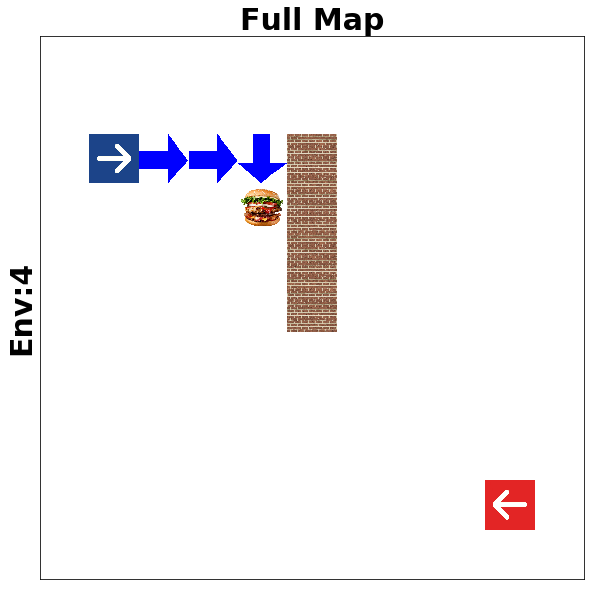
\includegraphics[scale=0.20]{figures/ENV:4_FM.png}}
\subfloat[]{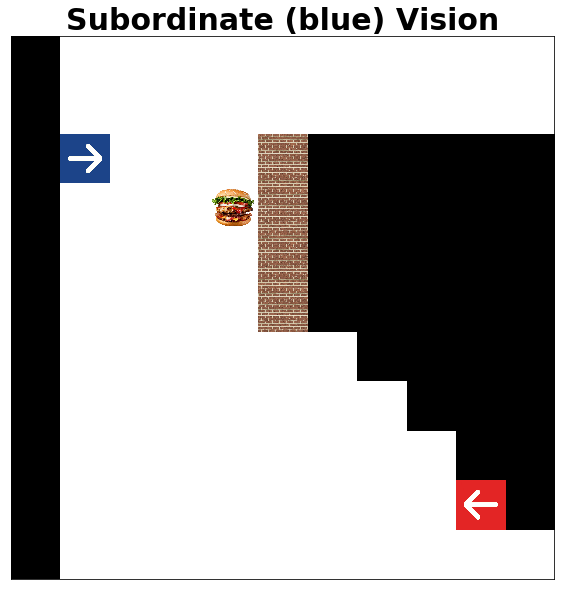
\includegraphics[scale=0.20]{figures/ENV:4_AI.png}}
\subfloat[]{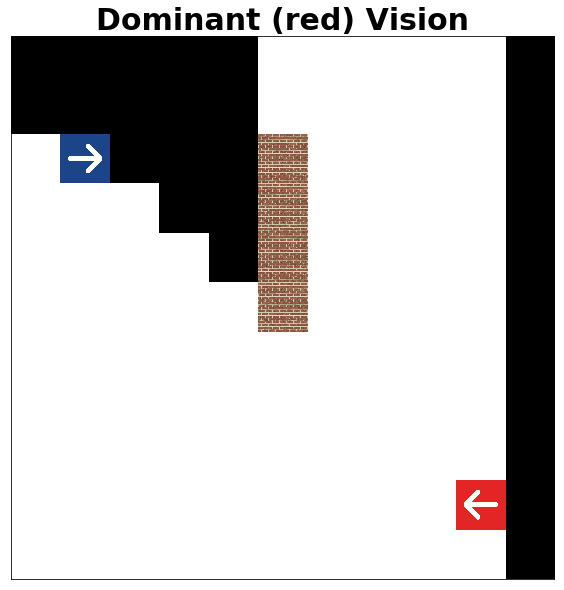
\includegraphics[scale=0.20]{figures/ENV:4_DM.png}}
\caption{Test  case 4: in this case the subordinate reached for the food. Although the dominant was looking toward the subordinate, the food was not visible for the dominant. This behavior matches what an agent with perspective taking would do.}
\label{fig.tc.4}
\end{center}
\end{figure}
\begin{figure}[H]
\begin{center}
\subfloat[]{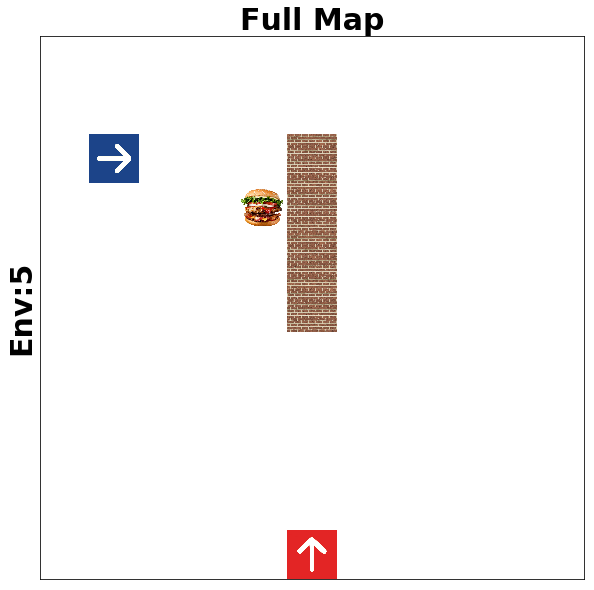
\includegraphics[scale=0.20]{figures/ENV:5_FM.png}}
\subfloat[]{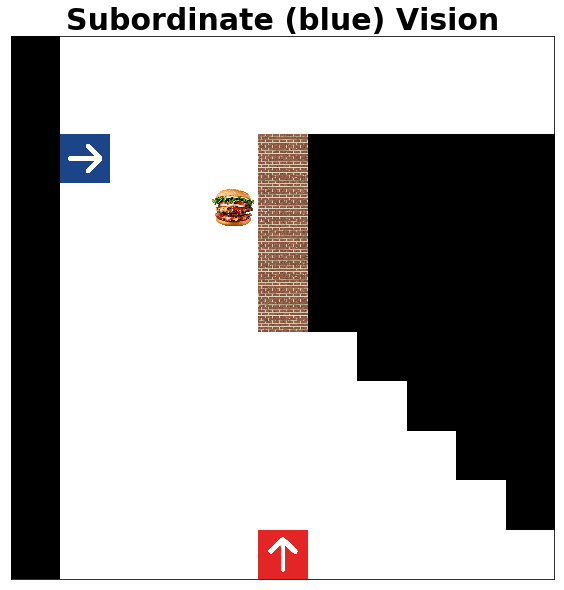
\includegraphics[scale=0.20]{figures/ENV:5_AI.png}}
\subfloat[]{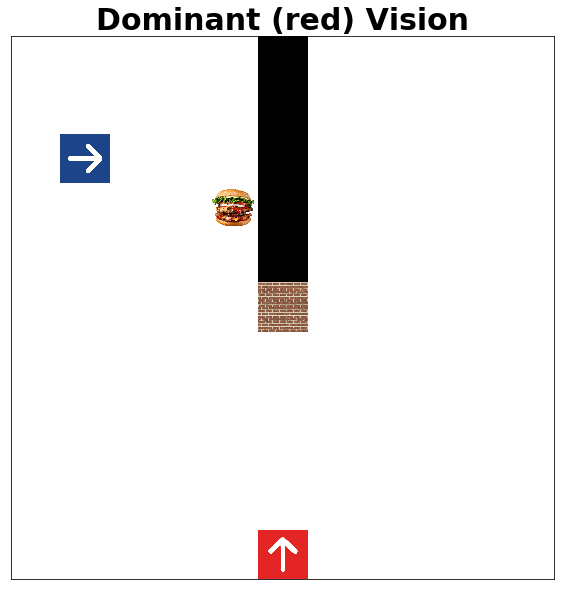
\includegraphics[scale=0.20]{figures/ENV:5_DM.png}}
\caption{test case 5, just like test case 2 but \(A_{dom}\) is farther away from food.}
\label{fig.tc.5}
\end{center}
\end{figure}

\begin{figure}[H]
\begin{center}
\subfloat[]{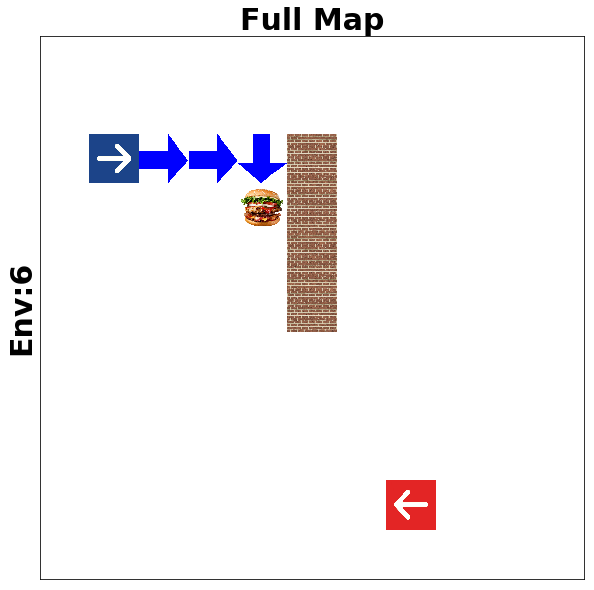
\includegraphics[scale=0.20]{figures/ENV:6_FM.png}}
\subfloat[]{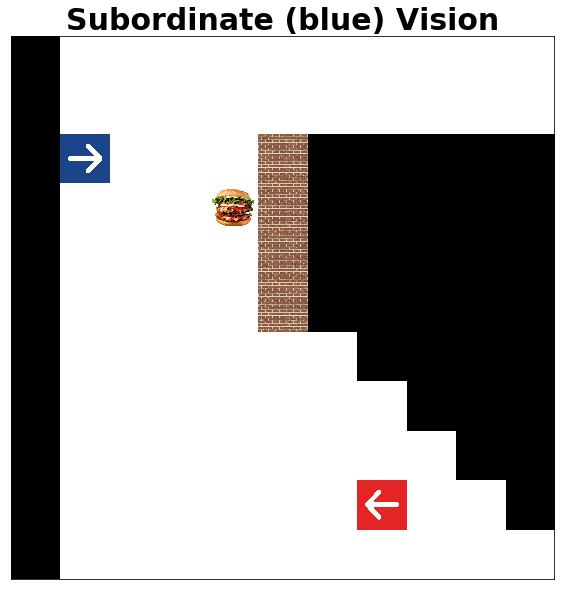
\includegraphics[scale=0.20]{figures/ENV:6_AI.png}}
\subfloat[]{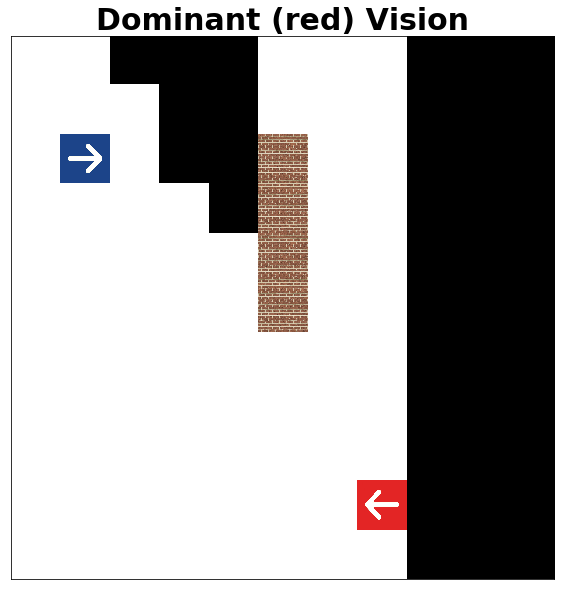
\includegraphics[scale=0.20]{figures/ENV:6_DM.png}}
\caption{Test  case 6: this test case is identical to test case 4 with the change in the distance between the dominant and the food. Although the dominant is closer to the food, it still cannot see it. The subordinate went for the food in this experiment which is a behavior to expect from an agent capable of perspective taking ability.}
\label{fig.tc.6}
\end{center}
\end{figure}



\begin{figure}[H]
\begin{center}
\subfloat[]{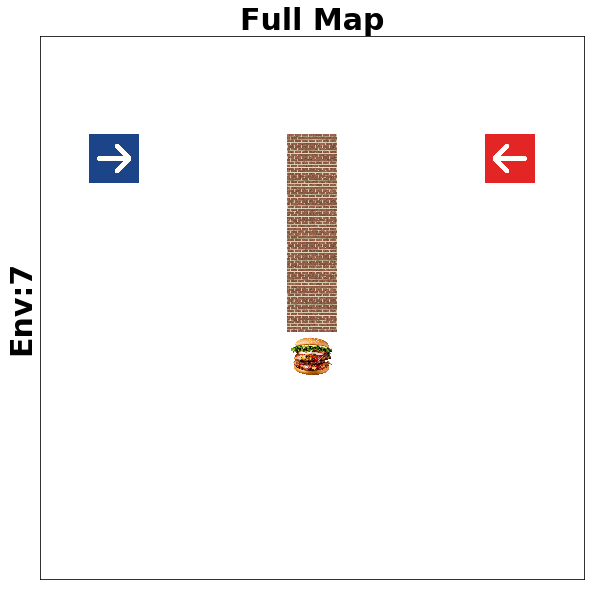
\includegraphics[scale=0.20]{figures/ENV:7_FM.png}}
\subfloat[]{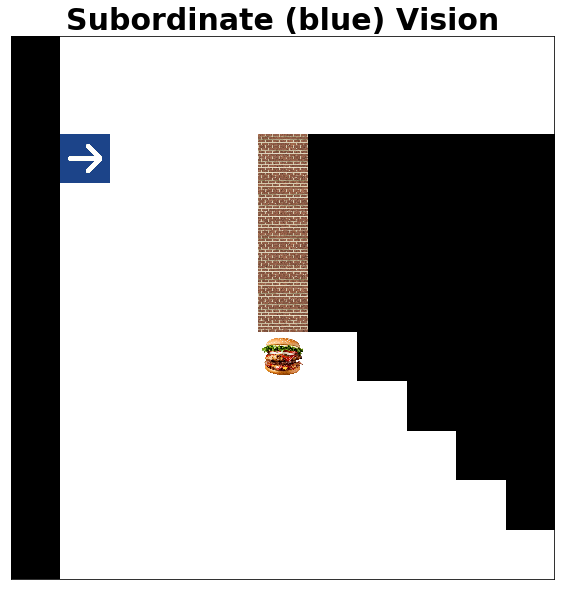
\includegraphics[scale=0.20]{figures/ENV:7_AI.png}}
\subfloat[]{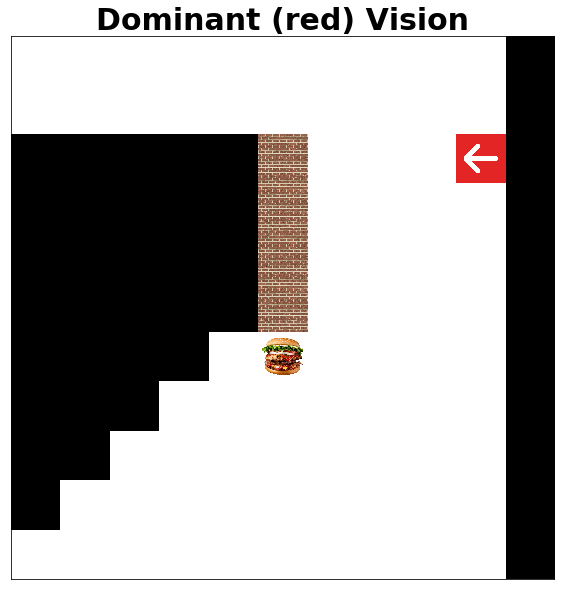
\includegraphics[scale=0.20]{figures/ENV:7_DM.png}}
\caption{\textbf {Test  case 7:} \(A_{sub}\) avoided the food although the dominant was not spotted in its field of view. It might be the case that food position is dangerous from previous experience while training.}
\label{fig.tc.7}
\end{center}
\end{figure}
\begin{figure}[H]
\begin{center}
\subfloat[]{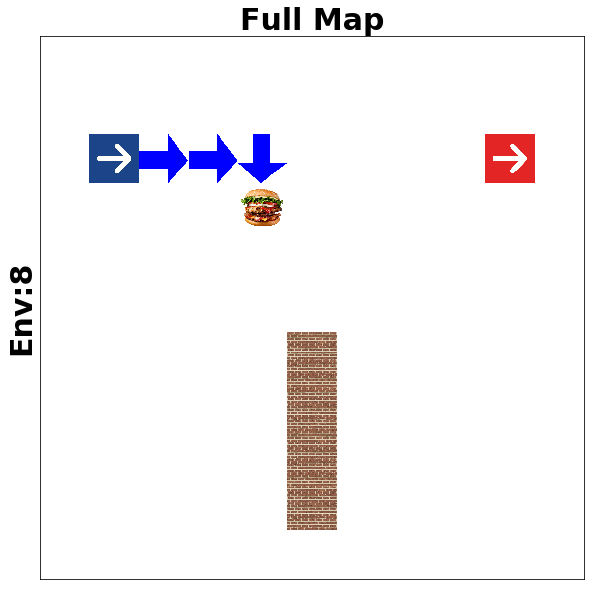
\includegraphics[scale=0.20]{figures/ENV:8_FM.png}}
\subfloat[]{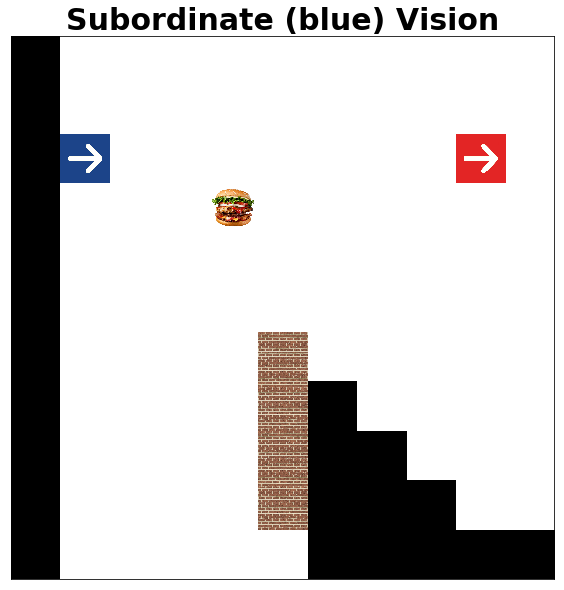
\includegraphics[scale=0.20]{figures/ENV:8_AI.png}}
\subfloat[]{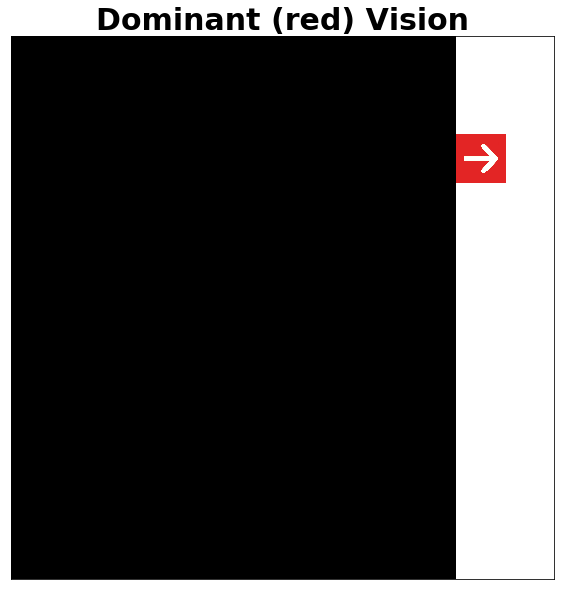
\includegraphics[scale=0.20]{figures/ENV:8_DM.png}}
\caption{Test  case 8: subordinate went for the food in this test case. Since the dominant was looking in the other direction, the food was not spotted by the dominant. Hence it is plausible to go for the food.  }
\label{fig.tc.8}
\end{center}
\end{figure}
\begin{figure}[H]
\begin{center}
\subfloat[]{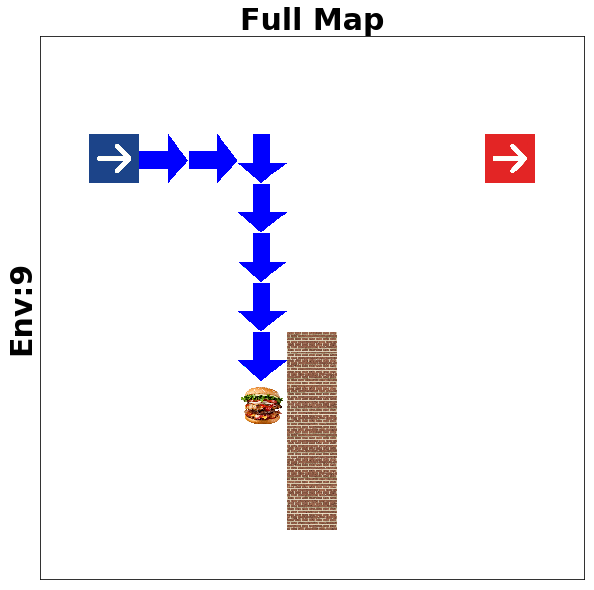
\includegraphics[scale=0.20]{figures/ENV:9_FM.png}}
\subfloat[]{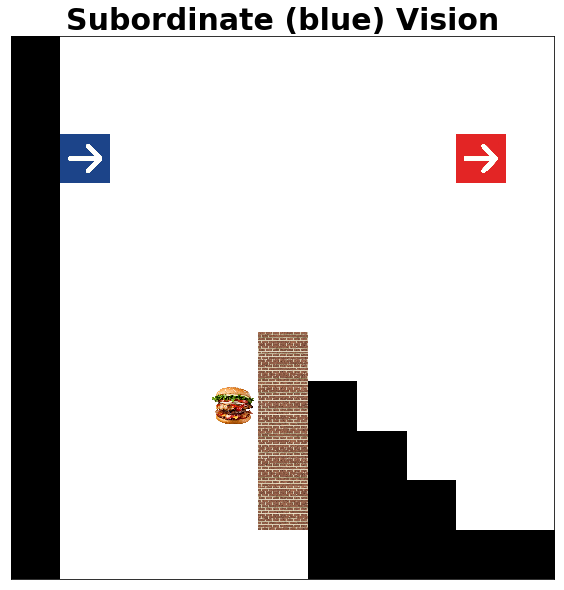
\includegraphics[scale=0.20]{figures/ENV:9_AI.png}}
\subfloat[]{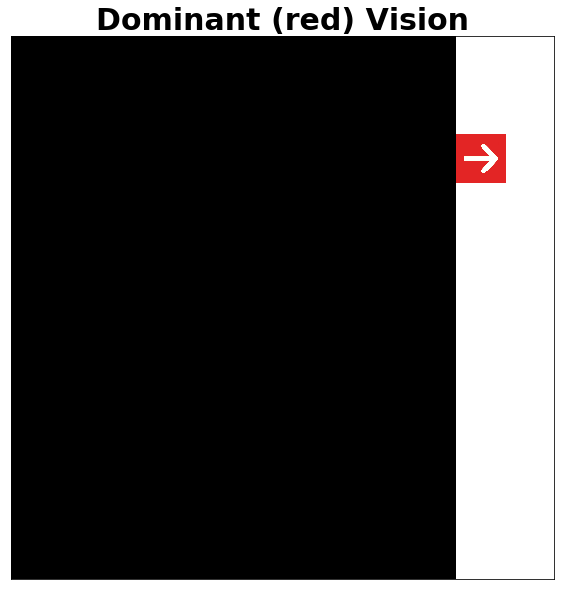
\includegraphics[scale=0.20]{figures/ENV:9_DM.png}}\\
\caption{Test  case 9: in this case we changed the food place and the obstacle where they are not seen by dominant. The subordinate retrieved the food successfully which is a behavior coincide with perspective knowledge.} 
\label{fig.tc.9}
\end{center}
\end{figure}
\begin{figure}[H]
\begin{center}
\subfloat[]{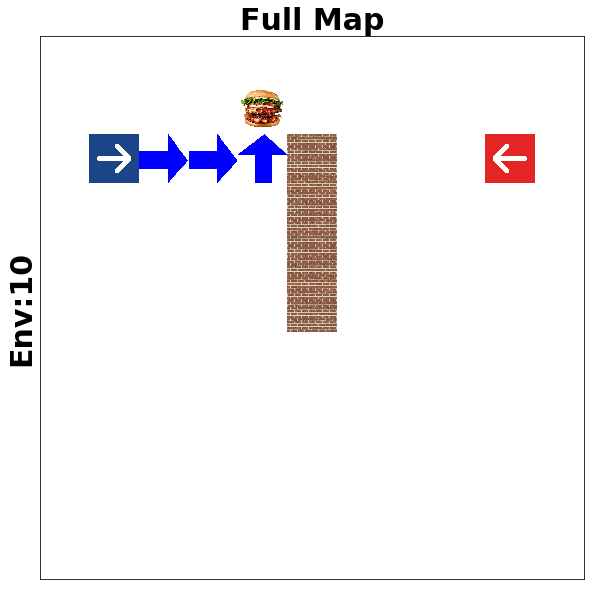
\includegraphics[scale=0.20]{figures/ENV:10_FM.png}}
\subfloat[]{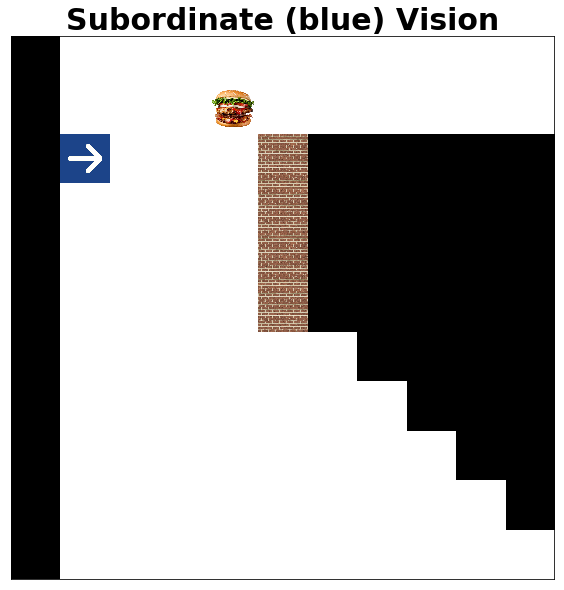
\includegraphics[scale=0.20]{figures/ENV:10_AI.png}}
\subfloat[]{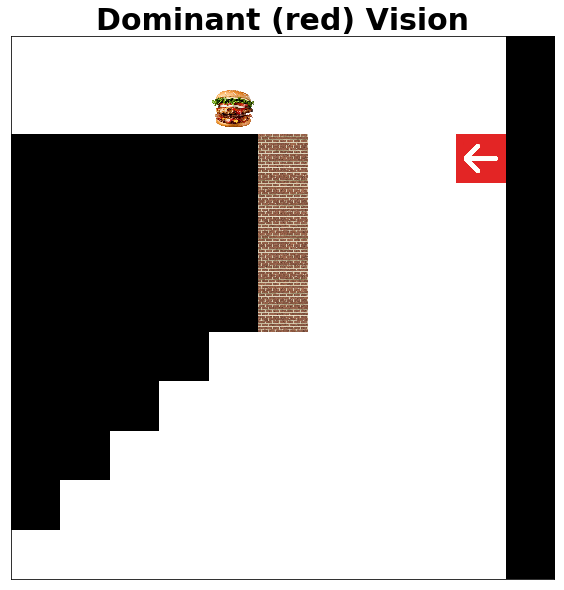
\includegraphics[scale=0.20]{figures/ENV:10_DM.png}}
\caption{Test  case 10: In this test case \(A_{sub}\) should or should not go to the food based on the trajectory followed. As we can see \(A_{dom}\) was never spotten by \(A_{sub}\).} 
\label{fig.tc.10}
\end{center}
\end{figure}

Our subordinate agent solved all of these test cases successfully demonstrating a capability for perspective taking. To control for the robustness of the results we included 4 sets of variations to the test cases where we shifted one or many elements by a pixel: 1- Shift all elements, 2- Shift dominant, 3- Shift Subordinate only, 4- Shift food position. In 95\% of these variations we observed similar results to the main results, hence confirming that our agent is not fooled by small variations of the data.

In table \ref{table:Tests} we summarize the results and show the expected behavior compared to the model behavior.
\begin{table}[H]
    \centering
    \begin{tabular}{|{c}||*{10}{c|}}
    \hline
    Test case&1&2&3&4&5&6&7&8&9&10\\
    \hline
    Video link&1&2&3&4&5&6&7&8&9&10\\
    \hline
    Figure&\ref{fig.tc.1}&\ref{fig.tc.2}&\ref{fig.tc.3}&\ref{fig.tc.4}&\ref{fig.tc.5}&
    \ref{fig.tc.6}&\ref{fig.tc.7}&\ref{fig.tc.8}&\ref{fig.tc.9}&\ref{fig.tc.10}\\
    \hline    
     \makecell{Dominant position \\ Food and obstacle \\ position}&DP&DP&DP&DP&DP&DP&FO&FO&FO&FO\\
    \hline
    \makecell{Expected behavior:\\Go or No}&Go&No&Go&Go&No&Go&No&Go&Go&Go\\
    \hline
    Actual behavior&Go&No&Go&Go&No&Go&No&Go&Go&Go\\
    \hline
    \end{tabular}
    \caption{show the test cases types (stabilizing everything but changing dominant position DP, or changing food and obstacle FO) and the expected behavior from the subordinate in each one. Last row show the actual behavior performed by the model.}
    \label{table:Tests}
\end{table}

\subsection{Inside the network}
The first step toward looking inside the network was checking T-SNE over the weights. In Figure (\ref{fig.TSNE_Weights}) we plot all the hidden nodes weights where we considered each hidden node a vector of length 633 (input size).
\begin{figure}[H]
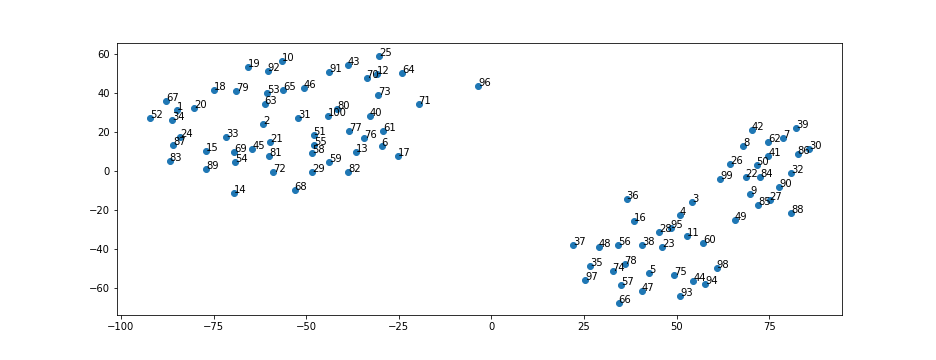
\includegraphics[scale=0.5,trim={3.5cm 0cm 2cm 0.5cm},clip]{figures/TSNE_Weights.png}
\caption{T-SNE over nodes in hidden layer, where we consider the weights from input are the node features.}
\label{fig.TSNE_Weights}
\end{figure}

Later we decided to check the most important neurons which basically hold highest weights. We took the neurons with highest weights that is connected to state value. Afterward we tried to see what those neurons represent, what areas they focus on and how much the dominant agent orientation important. To see these information we draw the weights between the inputs and those two neurons. \ref{fig.PN_61},\ref{fig.SN_61} show the neuron with highest positive weight and Figure \ref{fig.PN_76},\ref{fig.SN_76} show the neuron with highest negative weight. Those two neurons might be explained as desire for food and fear from dominant. 


\begin{figure}[H]
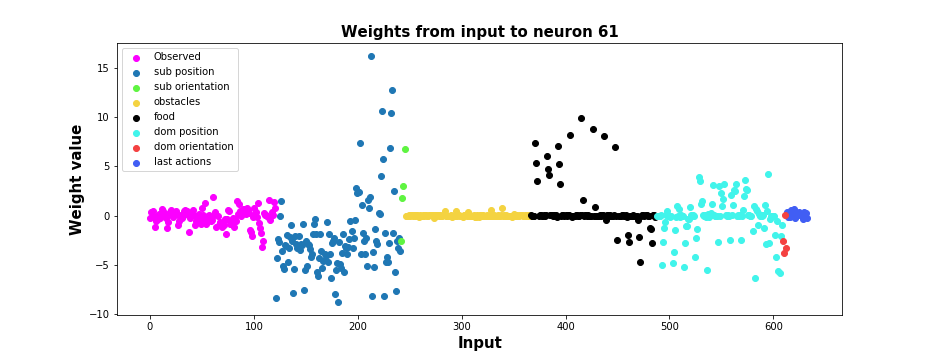
\includegraphics[scale=0.5,trim={3.5cm 0cm 2cm 0.5cm},clip]{figures/PN_61.png}
\caption{Each color represents one group of input e.g (observed area, \(A_{sub}\) position, food position etc..) as explained in section \ref{network.input}. The higher the value, the more weight is assigned to that specific input. A biological interpretation of neuron 61 might be the agent's desire for food.}
\label{fig.PN_61}
\end{figure}
\begin{figure}[H]
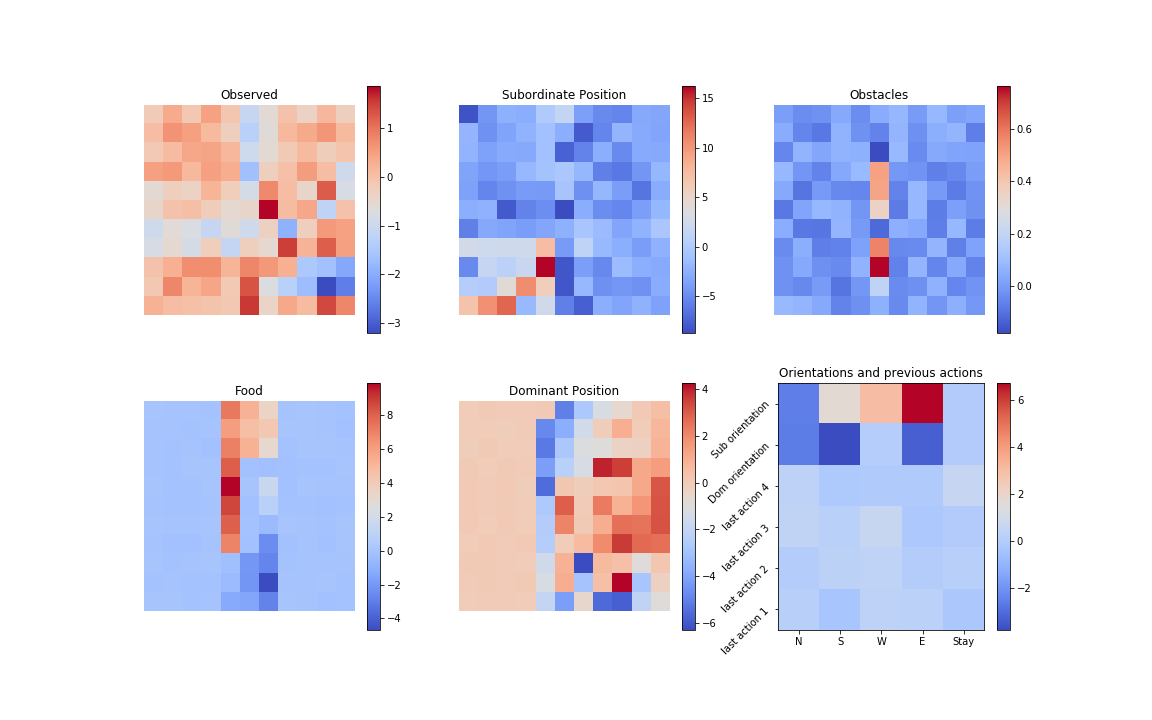
\includegraphics[scale=0.5,trim={5cm 2cm 4cm 3cm},clip]{figures/SN_61.png}
\caption{The weights between the input(\ref{network.input}) and neuron 61 in the hidden layer which hold the highest positive weight to state value node in the next layer. From this neuron we can see where our agent favor each element. We can notice in Food map, that the more food get close to dominant the less favorable it is because it means less probably to get it and more to get punished next to it. This neuron represent the desire for food. From dominant position map we can notice that this neuron give high values when dominant on the other side of the obstacle.}
\label{fig.SN_61}
\end{figure}
\begin{figure}[H]
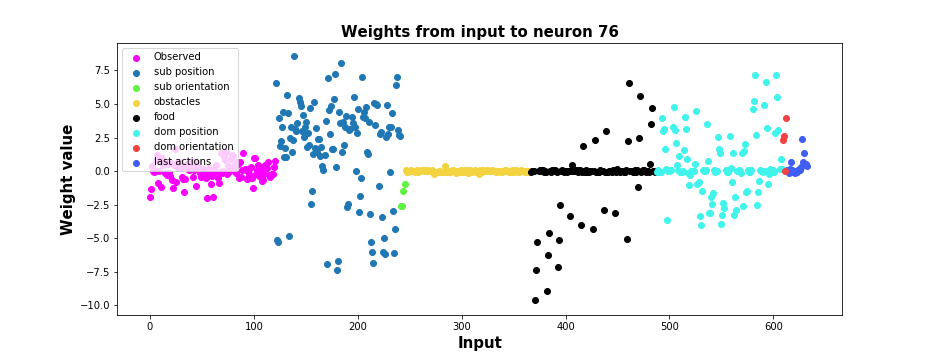
\includegraphics[scale=0.5,trim={3.5cm 0cm 2cm 0.5cm},clip]{figures/PN_76.png}
\caption{Each color represents one group of input e.g (observed area, \(A_{sub}\) position, food position etc..) as explained in section \ref{network.input}. The higher the value, the more weight is assigned to that specific input. A biological interpretation of neuron 76 might be the agent's fear from dominant.}
\label{fig.PN_76}
\end{figure}
\begin{figure}[H]
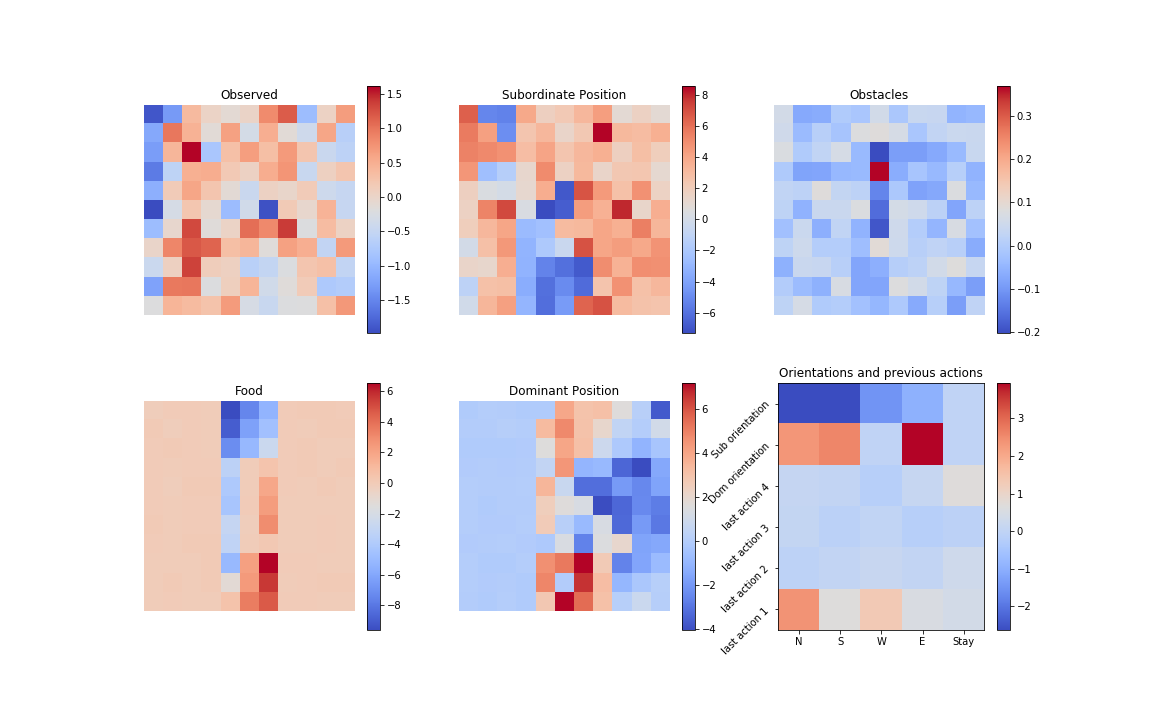
\includegraphics[scale=0.5,trim={5cm 2cm 4cm 3cm},clip]{figures/SN_76.png}
\caption{The weights between the input(\ref{network.input}) and neuron 76 in the hidden layer which hold the highest negative weight to state value node in the next layer. From this neuron we can see where our agent animus each element. We can notice in Food map, that the more food get close to dominant the more  animusable it is. Because it means less probability to get it and more to get punished next to it by dominant. This neuron represent the fear form dominant. From dominant position map we can notice that this neuron give high values when dominant around the obstacle. Which mean more probable negative reward for subordinate.}
\label{fig.SN_76}
\end{figure}
We recorded the hidden nodes values over those 10 cases with there variations. Afterward we applied T-SNE to draw the points in 2d. We can clearly see from Figure \ref{fig.expected.behavior}

\begin{figure}[H]
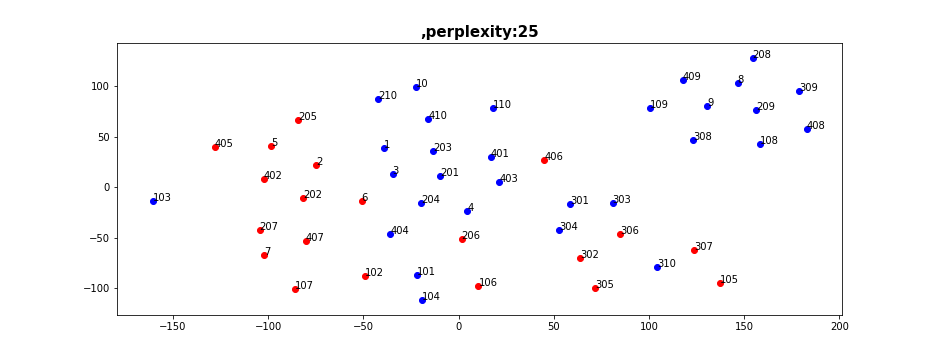
\includegraphics[scale=0.5,,trim={3.5cm , 1.5cm , 0cm , 0cm},clip]{figures/EB.png}
\caption{T-SNE over the activations over initial states for all 50 test cases. Blue: expected behavior is to go toward food, while red expected not to go toward food.}
\label{fig.expected.behavior}
\end{figure}
\begin{figure}[H]
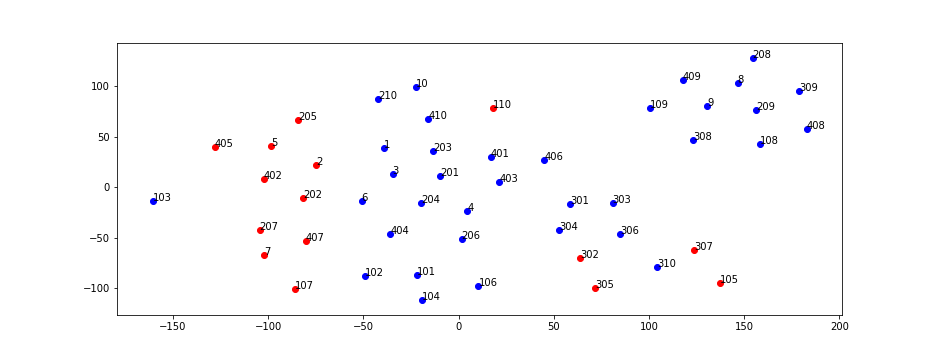
\includegraphics[scale=0.5,trim={3.5cm , 1.5cm , 0cm , 0cm},clip]{figures/AB.png}
\caption{T-SNE over the activations over initial states for all 50 test cases. Blue: went  to food, while red did not.}
\label{fig.actual.behavior}
\end{figure}

\section{Conclusion}
In this paper we showed 10 test cases that require perspective taking to be accomplished. Those test cases and their variations were solved by an artificial neural network trained with RL. The behavior of the agent showed evidence for basic perspective taking skills. By changing only the position of the dominant while keeping the positions of the subordinate, the food and the obstacle the same, we observed that the subordinate either went for the food or not depending on the position of the dominant as show in Figures (\ref{fig.tc.4},\ref{fig.tc.5}). Even when the dominant was in the field of view of the subordinate, the subordinate went for the food if the dominant could not see the food (test case 4, Figure (\ref{fig.tc.4}).  

We also presented a detailed analysis of the weights of the hidden layer and the activation over all the test cases with T-SNE. All T-SNE figures concluded to two clusters which make us believe that the network could be simplified even more. 

In the present work with relatively simple deep RL agents we observed that the subordinate agent can learn to take into account the behavior of the dominant agent through trial-and-error over a long training period. This is in stark contrast to chimpanzees who master the particular task in the first trial  (Hare et al 2000; 2001). However, it is important to note that the chimpanzees had learned about social hierarchies and about the behavior of other chimpanzees in their daily life over many years. Hence, the fact that in the present work the subordinate agents learned to take into account the behavior of the dominant agent demonstrates that at least part of perspective taking skills can indeed be learned through reinforcement learning. 

We are not claiming that RL would capture all aspects of perspective taking. We simply feel that by understanding the capabilities and limitations of RL agents in acquiring perspective taking we will better understand the computational demands of perspective taking and more generally, of mindreading, just as deep neural networks have led to a better understanding of vision (Aru \& Vicente, submitted).

In particular the current results show that for agents to show perspective taking behavior it is not needed to have a specific Theory of Mind module: aspects of mindreading, like perspective taking, can emerge through relatively simple RL algorithms. Through training these algorithms learn to take into account subtle cues about the relationships between the other agents and environmental cues like the position of food and obstacles. In many cases it might be that the position of the elements and orientation is sufficient for the agent to show behavior akin to perspective taking without any need for imagining what the dominant can or can not see. On the one hand it might seem that by studying such simple systems and environments we are missing the gist of human-like perspective taking. But, on the other hand, we would argue that we also need to understand these simpler cue-response contingencies underlying perspective taking. It is important to notice that perspective taking, like any other cognitive ability, has multiple facets and for the scientific understanding such abilities it is necessary to study all of these facets. Here we studied the simplest possible case where agents consisting of relatively simple neural networks learned with the help of reinforcement learning. In our future research we will test other architectures. One straightforward way for improving the present algorithm is to add external memory to the network to make it one step closer to brain. Another way is to incorporate a bias for learning about the other agent: while currently obstacles, food and the other agent were all equal for learning, we know that humans preferentially process signals coming from other humans (i.e. compared to pieces of furniture, falling leaves or sparrows). Endowing the agents with a bias to preferentially process inputs coming from the other agent could be an important step toward building AI agents with more complex mindreading skills (Aru \& Vicente, submitted).

In the end here lies the real advantage of AI research for understanding the brain: in artificial systems one can step-by-step make algorithms more complex and add different algorithms, while monitoring the performance at a particular task. In this fashion, part by part, algorithm by algorithm, it is easier to understand the emergence of complex cognitive functions underlying our intelligence.
\bibliographystyle{plain}
\bibliography{references}
\appendix
\section{Test cases}\label{test.cases}
% the \\ insures the section title is centered below the phrase: AppendixA
Backup test case with subordinate in different position.
\begin{figure}
    \centering
    \subfloat[]{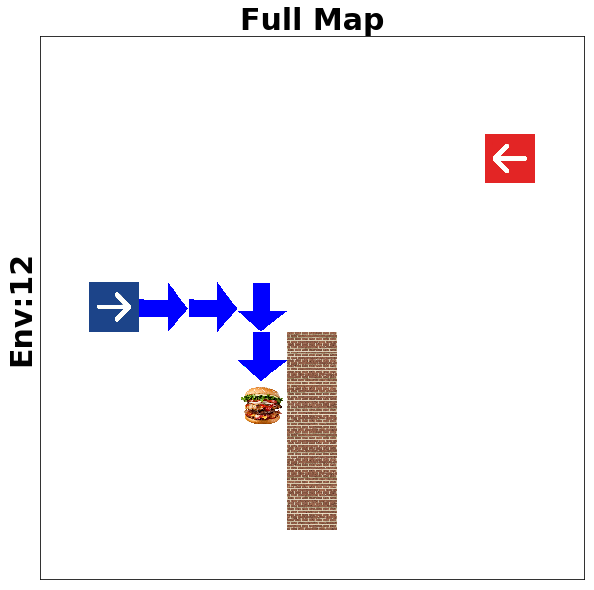
\includegraphics[scale=0.20]{figures/ENV:12_FM.png}}
    \subfloat[]{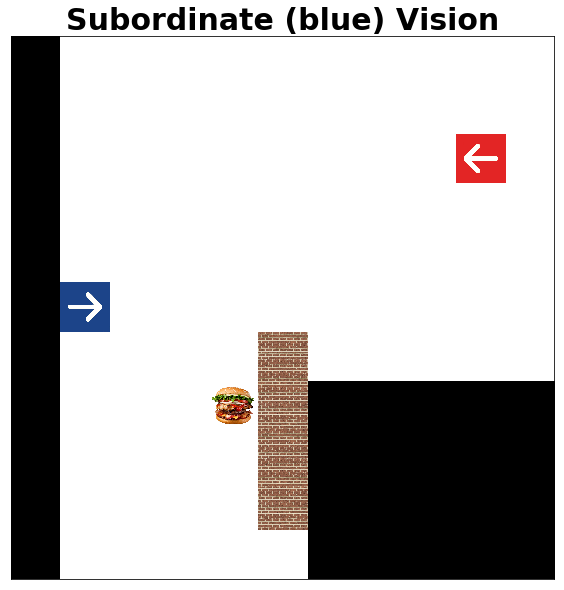
\includegraphics[scale=0.20]{figures/ENV:12_AI.png}}
    \subfloat[]{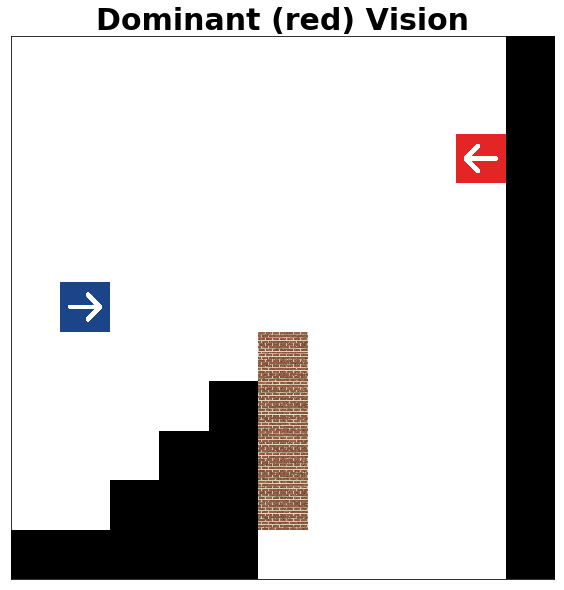
\includegraphics[scale=0.20]{figures/ENV:12_DM.png}}
    \caption{\textbf {Test  case 12:} \(A_{sub}\) can see the food and \(A_{dom}\) where the last can not see the food. \(A_{sub}\) go to food with the arrows trajectory.}
    \label{fig.tc.12}
\end{figure}
\section{Title of Appendix B}
% the \\ insures the section title is centered below the phrase: Appendix B

Text of Appendix B is Here
\end{document}
